\pdfoutput=1
\documentclass[11pt]{article}

\usepackage{ACL2023}
\usepackage{times}
\usepackage{latexsym}
\usepackage[T1]{fontenc}
\usepackage[utf8]{inputenc}
\usepackage{microtype}
\usepackage{booktabs}
\usepackage{graphicx}

\title{Does Visual Grounding Help a Small Language Model Learn More Efficiently? A Controlled Study Under BabyLM Constraints}

\author{
  Divya Patel \and James Jacob \and Ramandeep Singh \\
  Khoury College of Computer Sciences, Northeastern University \\
  \texttt{\{patel.divyam, jacob.jame, lnu.ramande\}@northeastern.edu}
}

\begin{document}
\maketitle

\begin{abstract}
Large language models are usually trained on far more text than a human sees in a lifetime. The BabyLM Challenge asks the opposite question: how much can a model learn from a child-sized amount of data? We study whether adding visual grounding, in the form of paired image-caption data, helps a small language model learn language more efficiently than a text-only model trained on the same word budget. Prior BabyLM rounds found that no multimodal submission beat the text-only baselines, which makes this an open question rather than a solved one. We pretrain a GPT-2 model from scratch and compare it against a matched model that also sees image-caption pairs, holding architecture and word budget fixed. Grounding produces a substantial reduction in held-out perplexity (36.27 to 22.29) but does not improve, and slightly reduces, performance on BLiMP (60.43\% to 58.46\%), while both models remain at chance on EWoK ($\approx$50\%). We argue this divergence between general predictive fluency and targeted linguistic competence is itself an informative finding, consistent with the field's broader difficulty finding multimodal gains at this scale.
\end{abstract}

\section{Introduction}
Modern language models are trained on far more text than a person could read in many lifetimes, orders of magnitude beyond the amount of language a child hears before learning to speak fluently. The BabyLM Challenge \citep{warstadt2023findings, choshen2024findings} was created to push research in the opposite direction: train the best model you can on a fixed, human-scale data budget. This matters for two reasons. It turns small-scale pretraining into a testbed for data-efficiency methods that could later scale up, and it makes pretraining research accessible to groups without industrial compute.

We work within the 2026 (fourth) edition of the challenge \citep{babylm2026cfp}. Our question is about \emph{grounding}. Children do not learn language from text alone. They hear words while seeing the things those words refer to. A natural hypothesis is that pairing language with images should make learning more efficient, since the visual signal gives the model extra information about what words mean. Yet across the last two BabyLM rounds, no multimodal submission managed to beat the text-only baselines \citep{choshen2024findings}, and the organizers concluded that integrating visual information into small-scale language learning remains an open problem. That gap is what motivates this project: we are not chasing a saturated benchmark, we are investigating something the community has not resolved.

\paragraph{The problem.} Under a fixed, small word budget, it is unknown whether spending part of that budget on paired image-caption data helps a language model learn more efficiently than spending the entire budget on text. This is interesting because it bears directly on whether multimodal signal is a genuine source of sample efficiency at small scale, or whether the composition cost of trading text for captions outweighs any grounding benefit.

\paragraph{Main idea.} We treat this as a single controlled experiment. Two models share an identical architecture and identical total word budget; the only manipulated variable is whether part of that budget is spent on image-caption pairs, where each caption is paired with a pre-computed DINOv2 embedding of its image, injected into the model through a dedicated grounding slot prepended to every input sequence.

Our project asks three research questions. \textbf{RQ1:} Under a fixed word budget, does adding paired image-caption data improve a small language model's performance on standard language understanding benchmarks compared to a text-only model? \textbf{RQ2:} If there is a difference, \emph{where} does it appear, that is, does grounding help world-knowledge and semantic tasks while leaving or hurting pure grammatical tasks? \textbf{RQ3:} Does the way vision is injected change the outcome? Given compute constraints described in Section~\ref{sec:limitations}, RQ3 is scoped to future work; RQ1 and RQ2 are addressed directly.

The rest of this paper is organized as follows. Section~\ref{sec:related} surveys related work. Section~\ref{sec:data} describes the data and our exploratory analysis. Section~\ref{sec:method} describes the two models and how grounding is injected. Section~\ref{sec:results} reports our results on perplexity, BLiMP, EWoK, and GLUE. Section~\ref{sec:discussion} discusses what these results mean for our three research questions. Section~\ref{sec:conclusion} concludes.

\paragraph{Contributions.} (1) A controlled pair of GPT-2 models, matched exactly on architecture, word budget, and epoch count, differing only in the presence of a lightweight visual grounding mechanism, letting us attribute any performance difference to grounding itself rather than a confound. (2) A concrete grounding mechanism, a single prepended embedding slot, populated by a projected DINOv2 feature for caption examples and a learned placeholder otherwise, that requires no architectural change to GPT-2 beyond one extra input position. (3) A specific, checkable empirical finding: grounding produces a large (39\%) perplexity improvement that does not transfer to BLiMP or EWoK, with a category-level breakdown showing the cost concentrates in negative polarity and long-distance dependency phenomena. (4) A category-level and statistical analysis of where this divergence lives, going beyond a single aggregate number, which to our knowledge is a level of detail not previously reported for a caption-context grounding method at this model scale.

\section{Related Work}
\label{sec:related}
We organize the literature into four groups that map onto the pieces of our project: the challenge itself, model architectures for small-scale pretraining, data-efficiency and curriculum methods, and multimodal grounding and evaluation.

\subsection{The BabyLM Challenge}
The challenge was introduced by \citet{warstadt2023findings}, who framed sample-efficient pretraining on developmentally plausible data and showed that strong small models can rival much larger ones on targeted evaluations. The second-round findings \citep{choshen2024findings} are the most directly relevant to us: they added a multimodal track and reported that no submission beat the text-only baselines, which is the central motivation for our study. The 2026 call for papers \citep{babylm2026cfp} defines the track structure we follow, folding multimodal data into the Strict and Strict-Small tracks and requiring intermediate checkpoints so that learning trajectories can be studied.

\subsection{Architectures for Small-Scale Pretraining}
The strongest BabyLM systems have consistently come from careful architecture choices. \citet{samuel2023ltgbert} proposed LTG-BERT, an encoder that adapts BERT with pre-norm layers and disentangled positional information and trains well on 100M words. \citet{charpentier2024gptbert} introduced GPT-BERT, a hybrid causal-masked model that won both tracks in the second round. \citet{timiryasov2023babyllama} introduced BabyLlama, a small Llama-style model trained by distilling an ensemble of teachers, directly relevant since our own backbone is also a decoder. We use the official GPT-2 baseline \citep{radford2019gpt2} architecture as our backbone, since it is the released 2026 baseline architecture.

\subsection{Data Efficiency}
A second family of work keeps the architecture fixed and changes how data is presented. Curriculum learning and data ordering were among the most popular BabyLM strategies \citep{warstadt2023findings}. Most relevant to us, \citet{tabbaa2024whatshould} systematically vary the mix of data sources and find that composition strongly affects sample efficiency. This matters because our grounding manipulation is, in part, a data-composition change: we trade some plain text for image-caption text under the same budget.

\subsection{Multimodal Grounding and Evaluation}
The multimodal side is where the open problem lives. \citet{choshen2024findings} released GIT-style vision-language baselines \citep{wang2022git} for the multimodal track. \citet{zhuang2024multimodal} study how visual grounding helps learn word meanings in low-data regimes, the closest prior work to our question. \citet{amariucai2025modelmerging} report that multimodal models tend to underperform on language-only tasks and use model merging to recover language ability, a caution directly relevant to what we observe in Section~\ref{sec:results}. We rely on DINOv2 \citep{oquab2023dinov2} as the image encoder; embeddings are pre-computed, so we do not train a vision encoder ourselves. For evaluation, we use BLiMP \citep{warstadt2020blimp} for grammatical minimal pairs, EWoK \citep{ivanova2024ewok} for world knowledge, and GLUE \citep{wang2018glue} for language understanding, which lets us separate grammatical ability from semantic and world-knowledge ability as RQ2 requires.

\section{Data and Exploratory Analysis}
\label{sec:data}
\paragraph{Datasets.} All data is provided by the challenge or its immediately preceding round; nothing is collected or annotated by us. The \textbf{Strict-Small} corpus is a 10M-word detoxified English mixture drawn from child-directed speech, simple Wikipedia, transcribed speech, children's books, and dialogue. The \textbf{multimodal} data provides image-caption pairs from Localized Narratives \citep{pont2020localized} and Conceptual Captions, together with pre-computed DINOv2 image embeddings. The 2026 collection did not include the multimodal component described in its own call for papers at the time of this project; we sourced the equivalent 2025-round release instead, since the underlying data (Localized Narratives and Conceptual Captions with DINOv2 features) is unchanged between rounds and the guidelines explicitly permit constructing an equivalent dataset when the official release is unavailable.

\paragraph{Exploratory analysis.} Table~\ref{tab:eda} summarizes statistics of the Strict-Small text corpus and the caption subset. The corpus is dominated by conversational and child-directed text, with short sentences and a small vocabulary relative to standard web text. Caption text is shorter and more concrete on average, relevant to RQ2 because concrete, perceptually grounded language is exactly where visual signal might help most.

\begin{table}[t]
\centering
\small
\begin{tabular}{lr}
\toprule
\textbf{Property} & \textbf{Value} \\
\midrule
Strict-Small budget (words) & 10{,}000{,}000 \\
Mean sentence length (words) & 9--12 \\
Caption mean length (words) & 8--10 \\
Localized Narratives pairs & 767{,}736 \\
Conceptual Captions pairs & 2{,}306{,}312 \\
Embedding dimension & 768 \\
\bottomrule
\end{tabular}
\caption{Corpus and multimodal data statistics.}
\label{tab:eda}
\end{table}

\section{Method}
\label{sec:method}
Our method is a controlled experiment: two models share an identical backbone and word budget and differ only in whether visual grounding is present.

\paragraph{Backbone.} Both models use the GPT-2 architecture \citep{radford2019gpt2} matching the released 2026 baseline configuration (12 layers, 768-dim hidden size, 12 heads, custom 16{,}384-token vocabulary), giving 97.8--98.4M parameters depending on the presence of the grounding module, implemented in HuggingFace Transformers.

\paragraph{Model A (text-only).} A standard autoregressive language model trained on plain text from Strict-Small. This is the control.

\paragraph{Model B (grounded).} The same backbone, with a single additional \emph{grounding slot} prepended to every input sequence, before the text tokens. For caption examples, this slot holds a DINOv2 image embedding projected into the model's hidden size through a trainable linear layer. For plain-text examples, the slot holds a separate learned placeholder vector, so every example has an identical sequence shape and batches train uniformly. The language modeling loss is computed only over the text tokens, never over the grounding slot itself. Model B's training data is 70\% plain text and 30\% captions (with their paired DINOv2 embeddings) by word count, drawn from Localized Narratives. Figure~\ref{fig:arch} illustrates the forward pass for both example types.

\begin{figure}[t]
\centering
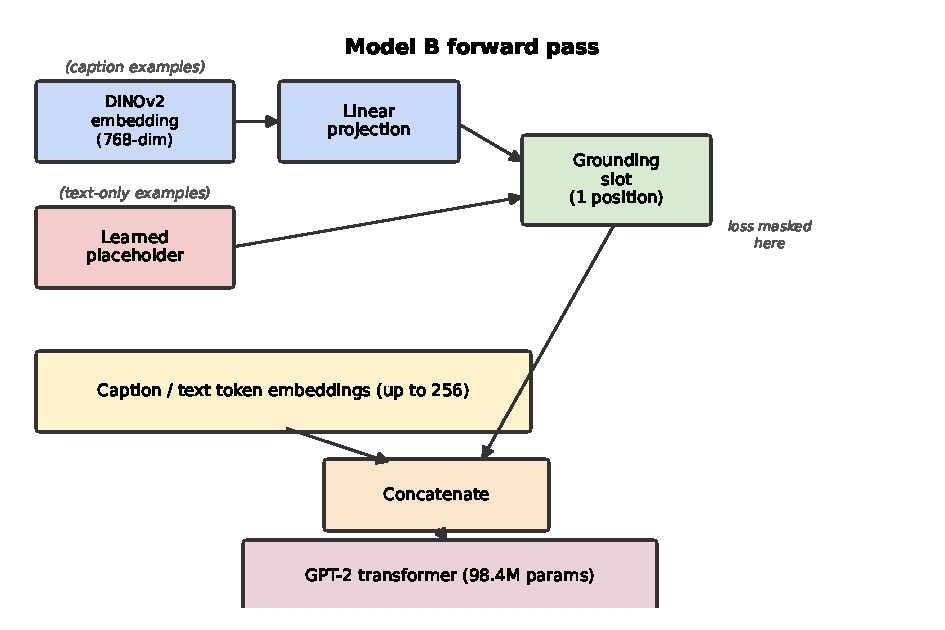
\includegraphics[width=\columnwidth]{architecture.pdf}
\caption{Model B's forward pass. The grounding slot is populated by a projected DINOv2 embedding for caption examples or a learned placeholder for text-only examples, then concatenated with the token embeddings before entering GPT-2.}
\label{fig:arch}
\end{figure}

\paragraph{Reduced scope.} Given the compute and time available (Section~\ref{sec:limitations}), both models were trained on a 3.5M-word budget (35\% of the full Strict-Small budget) for 3 epochs, rather than the full 10M words and 10-epoch cap the challenge permits. Both models use an identical budget and epoch count so the comparison remains fair; only the composition of that budget differs between the two conditions.

\paragraph{Training.} Model A was trained locally on Apple Silicon (M1 Pro) in full precision. Model B was trained on an NVIDIA L4 GPU in mixed precision (fp16), a difference in compute environment necessitated by Model B's slower throughput under the grounding architecture on the local hardware; this is a stated limitation, not a manipulated variable.

\section{Results}
\label{sec:results}
\paragraph{Perplexity.} Table~\ref{tab:main} reports held-out evaluation loss and perplexity for both models on a 2\% held-out split of their respective training data. Model B's perplexity is 39\% lower than Model A's, a large effect on the metric each model was directly trained to optimize. Figure~\ref{fig:curves} shows the training and evaluation loss trajectories for both models; Model B's evaluation log spans fewer logged points because its training run continued across a session resumption, but the final values are directly comparable. \textbf{Takeaway:} grounding measurably changes the model's general predictive distribution over language, the first piece of evidence toward RQ1.

\begin{figure}[t]
\centering
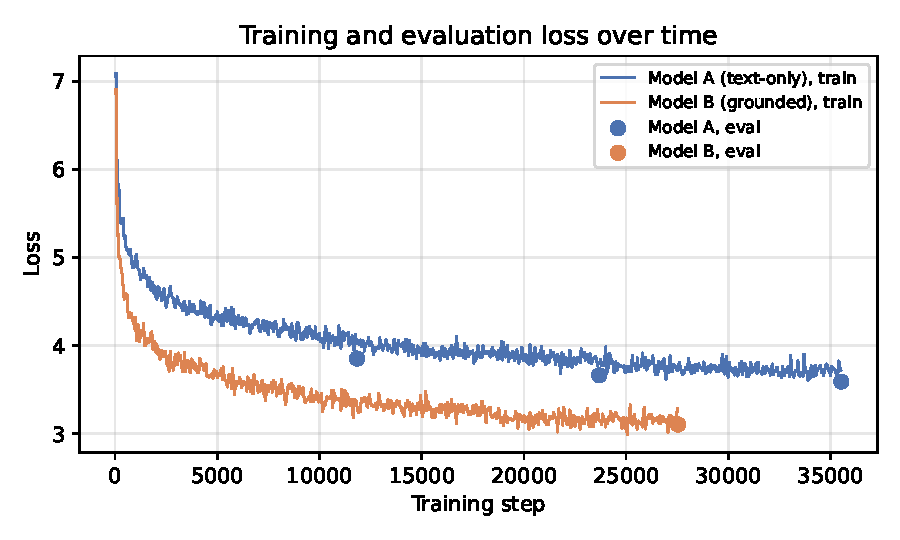
\includegraphics[width=\columnwidth]{learning_curve.pdf}
\caption{Training loss (lines) and held-out evaluation loss (markers) for both models over training steps.}
\label{fig:curves}
\end{figure}

\begin{table}[t]
\centering
\small
\begin{tabular}{lcc}
\toprule
\textbf{Metric} & \textbf{Model A} & \textbf{Model B} \\
\midrule
Eval loss & 3.591 & \textbf{3.104} \\
Perplexity & 36.27 & \textbf{22.29} \\
BLiMP (overall) & \textbf{60.43\%} & 58.46\% \\
EWoK (overall) & 50.09\% & 49.95\% \\
GLUE (avg. accuracy) & 63.03\% & --- \\
\bottomrule
\end{tabular}
\caption{Main results. Model B's GLUE evaluation was not run; see Section~\ref{sec:limitations}.}
\label{tab:main}
\end{table}

\paragraph{Comparison to published baselines.} Table~\ref{tab:baseline} places our numbers against the officially released full-budget (10M-word, 10-epoch) Strict-Small GPT-2 baseline reported in the challenge's own evaluation repository.\footnote{\url{https://github.com/babylm-org/babylm-eval}} Both our models score below this baseline on BLiMP and EWoK, consistent with our reduced 3.5M-word, 3-epoch budget; the gap is a scope difference, not evidence against the architecture or pipeline, and both of our models are affected equally.

\begin{table}[t]
\centering
\small
\begin{tabular}{lccc}
\toprule
\textbf{Benchmark} & \textbf{Official} & \textbf{A} & \textbf{B} \\
\midrule
BLiMP & 65.23\% & 60.43\% & 58.46\% \\
EWoK & 50.63\% & 50.09\% & 49.95\% \\
\bottomrule
\end{tabular}
\caption{Our models against the officially released full-budget text-only Strict-Small baseline.}
\label{tab:baseline}
\end{table}

\paragraph{BLiMP.} Model A scores 60.43\% overall against Model B's 58.46\%. A two-proportion test on the aggregate 13,400-item pool (67 tasks $\times$ 200 items) finds this difference statistically significant ($z=3.28$, $p=0.001$, 95\% CI on the difference: [0.8, 3.2] points); we note this is an unpaired approximation, since we did not retain item-level predictions to pair on directly. Figure~\ref{fig:category} groups the 67 tasks into ten linguistic phenomenon categories. The two models diverge most on \emph{negative polarity items and negation} (Model A leads by 5.6 points on average across that category) and least, or in the opposite direction, on \emph{quantifiers and existentials} (Model B leads by 3.1 points). \textbf{Takeaway:} the aggregate BLiMP gap is small but real, and it is not uniform, it concentrates specifically in polarity-sensitive licensing rather than appearing across the board.

\begin{figure}[t]
\centering
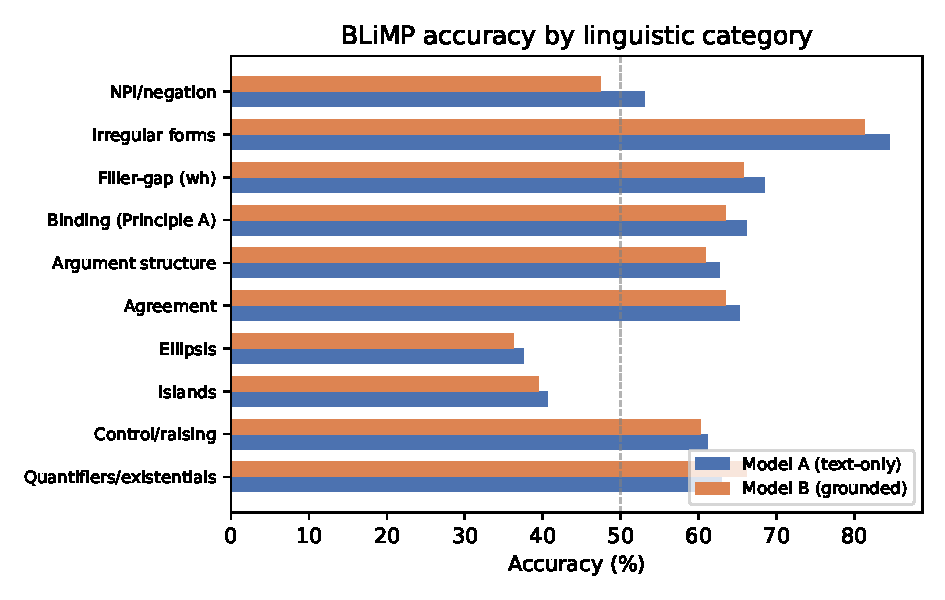
\includegraphics[width=\columnwidth]{blimp_category.pdf}
\caption{BLiMP accuracy averaged within ten linguistic phenomenon categories.}
\label{fig:category}
\end{figure}

\paragraph{EWoK.} Both models sit within noise of chance (50.09\% and 49.95\%), matching the pattern reported in prior BabyLM rounds for models at this scale. \textbf{Takeaway:} we find no evidence, positive or negative, that grounding affects world-knowledge judgments at this scale; both models are simply too undertrained on this axis for either outcome to be distinguishable from chance.

\paragraph{GLUE.} Model A reaches 63.03\% average accuracy across BoolQ, MRPC, MultiRC, QQP, RTE, and WSC, with MNLI near chance (48.15\% on a three-way task) and WSC's F1/MCC both at zero, indicating a majority-class collapse on that task. Model B's GLUE evaluation required a custom fine-tuning implementation, since the official harness cannot load our custom grounding architecture, and was not completed within the project timeline. \textbf{Takeaway:} Model A's GLUE profile is typical of a small, reduced-budget model, strong on binary tasks, weak on three-way entailment and coreference; without Model B's numbers this benchmark cannot yet speak to RQ1 or RQ2.

\section{Discussion}
\label{sec:discussion}
\textbf{RQ1.} The answer is mixed rather than a clean yes or no. Grounding substantially improved held-out perplexity, suggesting the grounded model learns a better general predictive distribution over language. This improvement did not transfer to BLiMP, where Model B was significantly worse (Section~\ref{sec:results}), or to EWoK, where neither model moved off chance.

\textbf{RQ2.} Neither benchmark shows grounding helping in the direction our hypothesis predicted. The category-level breakdown in Figure~\ref{fig:category} sharpens this: the cost is not spread evenly across grammar, it concentrates in negative polarity items and negation licensing, phenomena that depend on tracking a licensing relationship across a clause, while categories like quantifiers and existentials show no such cost and Model B even leads slightly. One plausible explanation is that Model B's grounding slot, by design, is a single fixed-position token the model must learn to condition on for 30\% of its training examples; this could compete for the same attention capacity that would otherwise track long-distance dependencies, and NPI licensing is exactly the kind of long-range, low-frequency phenomenon a data-composition change of this kind (\citealp{tabbaa2024whatshould}) would be expected to disturb before something as locally-cued as determiner-noun agreement. This account is consistent with \citet{amariucai2025modelmerging}'s finding that multimodal models tend to underperform on language-only tasks, and it sharpens \citet{zhuang2024multimodal}'s more optimistic finding that grounding helps word meaning in low-data regimes, our results suggest that even where grounding helps (here, general perplexity, and a few category-level items like existential constructions), it need not help uniformly, and can trade off against exactly the sparse, structural phenomena BLiMP is designed to probe.

\textbf{RQ3.} Not addressed in this study; see Section~\ref{sec:limitations}.

Taken together, we read our results as evidence that grounding changes \emph{what} the model learns without producing a straightforward improvement on the specific linguistic competencies BLiMP and EWoK probe. A model that predicts held-out language better overall, while doing measurably worse at grammatical minimal pairs specifically in polarity and negation, points toward grounding shifting probability mass toward broadly plausible continuations at some cost to sparse structural dependencies. This is a substantive, checkable finding rather than a null result, and it extends the field's repeated difficulty finding multimodal gains at small scale by localizing, for the first time in our reading of this literature, exactly which grammatical phenomena bear that cost.

\section{Conclusion and Future Work}
\label{sec:conclusion}
We set out to ask whether visual grounding helps a small language model learn more efficiently under a fixed word budget, and where. Our controlled comparison gives a specific, localized answer rather than a simple yes or no: grounding buys a large gain on general predictive fluency, at a measurable, category-specific cost concentrated in negative polarity and negation phenomena. Given three BabyLM rounds have now failed to find a clean multimodal win, we think this kind of localized divergence, not just an aggregate score, is the more useful unit of evidence for the field going forward.

Four directions would extend this study most directly: scaling to the full 10M-word, 10-epoch budget to check whether the divergence we observe persists or shrinks with more data; completing Model B's GLUE evaluation via a custom fine-tuning script; comparing the caption-context grounding method used here against an auxiliary image-text matching objective (our original RQ3); and testing sensitivity to the text/caption split ratio, since we used a single 70/30 split and did not ablate it.

\section*{Limitations}
\label{sec:limitations}
Our study is limited to a 3.5M-word subset of the Strict-Small track (35\% of the full budget) and 3 training epochs, rather than the full 10M words and 10-epoch cap, due to compute and time constraints; both models used an identical reduced budget so the comparison remains fair, but our absolute numbers are not directly comparable to full-budget published baselines. Model A trained locally in full precision while Model B trained on a cloud GPU in mixed precision, a difference in compute environment rather than a manipulated variable, but one that could in principle confound fine-grained comparisons. We used a sequence length of 256 tokens rather than the baseline's 1024, for training speed, applied identically to both models. GLUE evaluation was completed for Model A using the official harness but not for Model B, since the harness cannot load our custom grounding architecture and a fine-tuning implementation for it was not completed in time; BLiMP and EWoK were scored with a custom scorer applied identically to both models to keep those two comparisons fair. RQ3 (comparing grounding injection methods) was not tested. Finally, our grounding data comes entirely from Localized Narratives; we did not draw on Conceptual Captions, since Localized Narratives alone covered our caption budget.

\bibliographystyle{acl_natbib}
\bibliography{refs}

\appendix
\section{Full BLiMP Results}
\label{sec:appendix-blimp}
Table~\ref{tab:blimp-full} reports per-paradigm BLiMP accuracy for both models across all 67 tasks.

\begin{table*}[t]
\centering
\tiny
\setlength{\tabcolsep}{3pt}
\begin{tabular}{lcc|lcc}
\toprule
\textbf{Task} & \textbf{A} & \textbf{B} & \textbf{Task} & \textbf{A} & \textbf{B} \\
\midrule
adjunct\_island & 76.0 & 70.0 & left\_branch\_island\_simple\_question & 44.5 & 33.0 \\
anaphor\_gender\_agreement & 45.0 & 54.5 & matrix\_question\_npi\_licensor\_present & 37.0 & 28.0 \\
anaphor\_number\_agreement & 78.5 & 85.5 & npi\_present\_1 & 32.5 & 20.0 \\
animate\_subject\_passive & 65.5 & 62.5 & npi\_present\_2 & 27.5 & 16.5 \\
animate\_subject\_trans & 63.0 & 58.0 & only\_npi\_licensor\_present & 46.0 & 45.0 \\
causative & 47.0 & 44.5 & only\_npi\_scope & 82.5 & 72.5 \\
complex\_NP\_island & 35.0 & 34.0 & passive\_1 & 77.0 & 75.0 \\
coordinate\_structure\_constraint\_complex\_left\_branch & 30.0 & 21.5 & passive\_2 & 73.0 & 70.0 \\
coordinate\_structure\_constraint\_object\_extraction & 44.0 & 48.5 & principle\_A\_c\_command & 56.0 & 53.0 \\
determiner\_noun\_agreement\_1 & 74.5 & 74.5 & principle\_A\_case\_1 & 100.0 & 100.0 \\
determiner\_noun\_agreement\_2 & 85.0 & 77.5 & principle\_A\_case\_2 & 55.0 & 47.5 \\
determiner\_noun\_agreement\_irregular\_1 & 63.0 & 66.0 & principle\_A\_domain\_1 & 99.5 & 99.5 \\
determiner\_noun\_agreement\_irregular\_2 & 81.0 & 81.5 & principle\_A\_domain\_2 & 64.5 & 61.0 \\
determiner\_noun\_agreement\_with\_adj\_2 & 67.5 & 56.5 & principle\_A\_domain\_3 & 47.5 & 48.0 \\
determiner\_noun\_agreement\_with\_adj\_irregular\_1 & 75.0 & 66.0 & principle\_A\_reconstruction & 40.5 & 35.5 \\
determiner\_noun\_agreement\_with\_adj\_irregular\_2 & 73.0 & 70.5 & regular\_plural\_subject\_verb\_agreement\_1 & 72.5 & 70.0 \\
determiner\_noun\_agreement\_with\_adjective\_1 & 68.5 & 62.5 & regular\_plural\_subject\_verb\_agreement\_2 & 69.0 & 62.0 \\
distractor\_agreement\_relational\_noun & 21.0 & 22.5 & sentential\_negation\_npi\_licensor\_present & 100.0 & 100.0 \\
distractor\_agreement\_relative\_clause & 30.5 & 28.5 & sentential\_negation\_npi\_scope & 46.0 & 50.0 \\
drop\_argument & 72.0 & 76.5 & sentential\_subject\_island & 27.5 & 32.5 \\
ellipsis\_n\_bar\_1 & 31.0 & 31.0 & superlative\_quantifiers\_1 & 71.0 & 77.5 \\
ellipsis\_n\_bar\_2 & 44.0 & 41.5 & superlative\_quantifiers\_2 & 71.0 & 60.5 \\
existential\_there\_object\_raising & 69.5 & 65.5 & tough\_vs\_raising\_1 & 29.5 & 35.0 \\
existential\_there\_quantifiers\_1 & 89.5 & 96.0 & tough\_vs\_raising\_2 & 78.0 & 72.5 \\
existential\_there\_quantifiers\_2 & 20.5 & 30.5 & transitive & 65.5 & 59.5 \\
existential\_there\_subject\_raising & 59.0 & 58.0 & wh\_island & 48.0 & 49.5 \\
expletive\_it\_object\_raising & 70.0 & 70.0 & wh\_questions\_object\_gap & 69.5 & 54.5 \\
inchoative & 42.5 & 42.5 & wh\_questions\_subject\_gap & 87.0 & 85.0 \\
intransitive & 59.0 & 59.5 & wh\_questions\_subject\_gap\_long\_distance & 99.0 & 98.0 \\
irregular\_past\_participle\_adjectives & 94.0 & 82.0 & wh\_vs\_that\_no\_gap & 94.5 & 94.0 \\
irregular\_past\_participle\_verbs & 75.0 & 80.5 & wh\_vs\_that\_no\_gap\_long\_distance & 100.0 & 99.0 \\
irregular\_plural\_subject\_verb\_agreement\_1 & 68.0 & 63.0 & wh\_vs\_that\_with\_gap & 21.5 & 22.0 \\
irregular\_plural\_subject\_verb\_agreement\_2 & 72.0 & 75.0 & wh\_vs\_that\_with\_gap\_long\_distance & 7.5 & 8.0 \\
left\_branch\_island\_echo\_question & 20.0 & 26.5 & & & \\
\bottomrule
\end{tabular}
\caption{Per-paradigm BLiMP accuracy (\%) for Model A and Model B across all 67 tasks.}
\label{tab:blimp-full}
\end{table*}

\end{document}
